\vzmstitle{МОДЕЛЬ ОБОБЩЁННОГО ЛЮФТА В~УСЛОВИЯХ СТОХАСТИЧНОСТИ ОПРЕДЕЛЯЮЩИХ ПАРАМЕТРОВ}
\vzmsauthor{Борзунов}{С.\,В.}
\vzmsauthor{Семенов}{М.\,Е.}
\vzmsauthor{Мелешенко}{П.\,А.}
\vzmsauthor{Толкачев}{А.\,В.}
\vzmsinfo{Воронеж; {\it mkl150@mail.ru}}
\vzmscaption

Изучение и моделирование сложных технических систем приводит к необходимости представлять в формальном виде нелинейности гистерезисной природы. Многие физико"=химические, биологические и экономические системы\hspace{-0.9pt} демонстрируют гистерезисное поведение, что обуславливается либо их внутренней структурой, либо динамическими особенностями протекающих в таких системах процессов. Работа посвящена обобщению одной из основных моделей гистерезиса~--- люфта на класс преобразователей, характеристики которых определяются случайными параметрами.

Физическая модель люфта представляет собой систему, состоящую из цилиндра длины $h$ и поршня, которые могут перемещаться в горизонтальном направлении (см.~рис.~\ref{classical_backlash}\textit{а}). Положение цилиндра будем считать входной координатой, а положение поршня~--- выходной. Вход системы в зависимости от времени на конечном интервале $t\in[t_0,T]$ обозначим через $x(t)$, выход~--- через $u(t)$.

Для вещественных чисел $v_r,v_l \in \mathbb{R}$ рассмотрим \emph{определяющие кривые $\tilde{\varGamma}^{v_l}_l$, $\tilde{\varGamma}^{v_r}_r$ обобщённого люфта с параметрами сдвига $v_l,v_r$}. Такие кривые вводятся согласно правилам: $\tilde{\varGamma}^{v_l}_l\colon u_l(x)=l(x)+v_l$ и $\tilde{\varGamma}^{v_r}_r\colon u_r(x)=r(x)+v_r$. Здесь $l(x)$ и $r(x)$~--- функции, отражающие механизм передачи движения цилиндра на движение поршня. Предполагается, что функции $l(x)$ и $r(x)$ удовлетворяют глобальному условию Липшица на всей области определения и монотонно возрастают. Кроме того, пусть выполняется условие отсутствия пересечения положений границ люфта: $\forall x\;(l(x)>r(x))$. Для $v_r,v_l \in \mathbb{R}$, таких, что $l(w) + v_l > r(w)  +v_r $ для всех $w \in \mathbb{R}$, и для произвольной непрерывной функции $x : [t_0,T] \to \mathbb{R}$, и $x_0 := x(t_0)$ введём понятие обобщённого люфта. Выход $u(t)$ в каждый момент времени $t$ подчиняется операторному соотношению
\begin{equation*}
u(t) = \hat{L}_S[t_0, u_0; \tilde{\varGamma}_l^{v_l}, \tilde{\varGamma}_r^{v_r}]x(t),\quad t_0\leqslant t\leqslant T,\label{L_operator}\eqno{(1)}
\end{equation*}
где $t_0$~--- начальный момент времени, $u_0:=u(t_0)$~--- начальное значение функции выхода.

\begin{figure}[ht]
\begin{center}
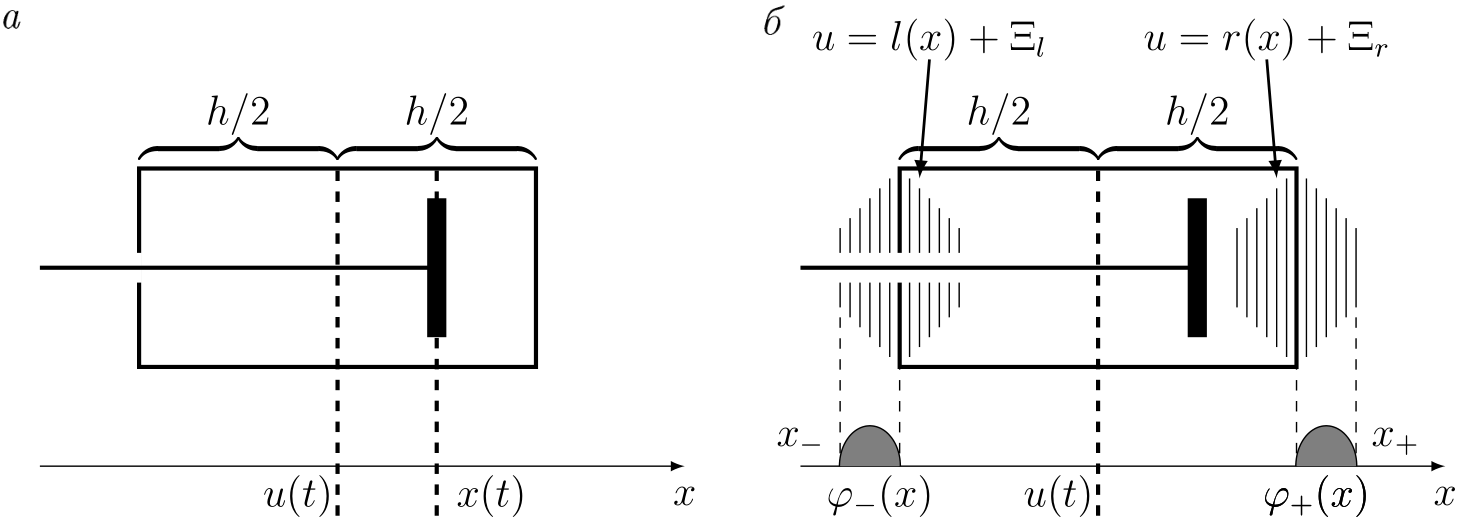
\includegraphics[width=0.75\textwidth]{vzms_2020.png}
\caption{Схематическое изображение люфта. Панель \textit{а})~--- люфт с детерминированными параметрами, \textit{б})~--- со стохастическими параметрами. Серой заливкой выделены области под кривыми\! $\varphi_l(z)$\! и\! $\varphi_r(z)$, определяющими плотность вероятности левой и правой границ цилиндра соответственно}\label{classical_backlash}
\end{center}
\end{figure}

Параметры носителей гистерезисных свойств могут испытывать изменения, связанные со старением материалов или варьироваться за счёт воздействия иных неконтролируемых факторов. В связи с этим возникает необходимость обобщения конструктивных моделей гистерезисных преобразователей, учитывающих вероятностный характер определяющих их параметров. Введём понятие недетерминированного обобщённого люфта. Если считать положения левой и правой стенок цилиндра распределёнными по случайному закону, то соответствующий преобразователь естественно назвать люфтом со случайными параметрами, или недетерминированным обобщённым люфтом. Предполагаются заданными функции $\varphi_l(x)$ и $\varphi_r(x)$, трактуемые как плотности вероятности, соответствующие положениям левой и правой границ цилиндра соответственно (см.~рис.~\ref{classical_backlash}\textit{б}). Выход пре\-об\-ра\-зо\-ва\-те\-ля"=люфта со случайными параметрами будем считать случайным процессом $u(t)$.

Следуя классической схеме~[1], определим выход на произвольных входах. Случайный процесс $u(t)$ в каждый момент времени $t$ подчиняется операторному соотношению
\begin{equation*}
u(t) = \hat{L}[t_0, u_0; \tilde{\varGamma}_l^{\Xi_l}, \tilde{\varGamma}_r^{\Xi_r}]x(t),\quad t_0\leqslant t\leqslant T,\eqno{(2)}\label{L_operator_stochastic}
\end{equation*}
где $x_0=x(t_0)$ и $u_0=u(t_0)$~--- начальные значения функций входа и выхода соответственно. Здесь $\tilde{\varGamma}_l^{\Xi_l}$, $\tilde{\varGamma}_r^{\Xi_r}$~--- определяющие кривые люфта, $\tilde{\varGamma}_l^{\Xi_l}\colon u_l=l(x)+\Xi_l$ и $\tilde{\varGamma}_r^{\Xi_r}\colon u_r=r(x)+\Xi_r$, $\Xi_l$, $\Xi_r$~--- случайные величины с плотностями вероятности $\varphi_l(x)$ и $\varphi_r(x)$ соответственно.

\textbf{Теорема.}
{\it Пусть на интервале $t_0\leqslant t\leqslant T$ имеет место равномерная сходимость последовательности кусочно"=монотонных функций $\{x_n(t)\}$, $n=1,2,\dots$, к функции} $x_{*}(t)$:
\begin{equation*}
x_{n}(t) \rightrightarrows x_{*}(t) \quad\forall t\in[t_0, T].\eqno{(3)}
\end{equation*}
{\it Тогда выход преобразователя представляет собой случайный процесс, сходящийся по распределению к случайному процессу}
\begin{equation*}
u_{*}(t) = \hat{L}[u_0, x_0; \tilde{\varGamma}_l^{\Xi_l}, \tilde{\varGamma}_r^{\Xi_r}]x_{*}(t).\eqno{(4)}
\end{equation*}



\hspace{-1.3pt}\textbf{Благодарности.}\hspace{-1pt} Исследование выполнено при финансо\-вой поддержке РФФИ (грант №19-08-00158-а) и РНФ (грант №19-11-00197).

% Оформление списка литературы
\smallskip \centerline {\bf Литература} \nopagebreak

1. {\it Красносельский М.А., Покровский А.В.} Системы с гистерезисом. М.: Наука, 1983. 272 с.
